\documentclass[journal]{IEEEtran}
\usepackage{amsmath,amsfonts}
\usepackage{array}
\usepackage{textcomp}
\usepackage{stfloats}
\usepackage{url}
\usepackage{verbatim}
\usepackage{graphicx}
\usepackage{cite}
\usepackage[margin=1in]{geometry}
\usepackage{xcolor}
\usepackage{pifont}
\usepackage{amssymb}
\usepackage{tabularx}
\usepackage{multirow}
\usepackage{booktabs}
\usepackage{placeins}
\usepackage{newfloat}
\usepackage{listings}
\setlength{\marginparwidth}{2cm}
\usepackage{todonotes}
\usepackage{amsmath}
% \usepackage{algorithm}
\usepackage{subcaption}
% \usepackage{algorithmic}
% \usepackage{algorithm2e}
\usepackage{algorithm}
\usepackage{algpseudocode}
\usepackage{amsmath}
% \hyphenation{op-tical net-works semi-conduc-tor IEEE-Xplore}
\usepackage{hyperref}
\usepackage[margin=1in]{geometry}
\usepackage{listings}
% Change 'Listing' to 'Algorithm'
\renewcommand{\lstlistingname}{Algorithm}

\begin{document}

\title{DenoMAE2.0: Improving Denoising Masked Autoencoders by Classifying Local Patches for Automatic Modulation Classification}

\author{Atik Faysal,~\IEEEmembership{Member,~IEEE}, 
Mohammad Rostami,~\IEEEmembership{Student Member,~IEEE},
Taha Boushine,~\IEEEmembership{Student Member,~IEEE},
Reihaneh Gh. Roshan,~\IEEEmembership{Student Member,~IEEE},
Huaxia Wang,~\IEEEmembership{Member,~IEEE},
Nikhil Muralidhar,~\IEEEmembership{Member,~IEEE},
Yu-Dong Yao,~\IEEEmembership{Fellow,~IEEE}
}

% The paper headers
\markboth{Journal of \LaTeX\ Class Files,~Vol.~14, No.~8, August~2021}%
{Shell \MakeLowercase{\textit{et al.}}: A Sample Article Using IEEEtran.cls for IEEE Journals}

% Remember, if you use this you must call \IEEEpubidadjcol in the second
% column for its text to clear the IEEEpubid mark.

\maketitle

\begin{abstract}

% We introduce DenoMAE2.0, an enhanced denoising masked autoencoder that integrates a local patch classification objective alongside traditional reconstruction loss to improve representation learning and robustness. Unlike conventional Masked Autoencoders (MAE), which focus solely on reconstructing missing inputs, DenoMAE2.0 introduces position-aware classification of unmasked patches, enabling the model to capture fine-grained local features while maintaining global coherence. This dual-objective approach is particularly beneficial in semi-supervised learning for wireless communication, where high noise levels and data scarcity pose significant challenges. We conduct extensive experiments on modulation signal classification across a wide range of Signal-to-Noise Ratios (SNRs), from extremely low to moderately high conditions and in a low data regime. Our results demonstrate that DenoMAE2.0 surpasses its predecessor, DenoMAE, and other baselines in both denoising quality and downstream classification accuracy. DenoMAE2.0 achieves a 1.1\% improvement over DenoMAE on our dataset and 11.83\%, 16.55\% significant improved accuracy gains on the RadioML benchmark, over DenoMAE, for constellation diagram classification of modulation signals. 

We introduce DenoMAE2.0, an enhanced denoising masked autoencoder designed to significantly improve representation learning for automatic modulation classification (AMC) in wireless communications. Unlike standard Masked Autoencoders (MAEs), which solely reconstruct masked inputs, DenoMAE2.0 jointly performs denoising and reconstruction by incorporating a position-aware local patch classification objective. This approach enables the model to simultaneously denoise corrupted signals and accurately reconstruct missing information, effectively capturing both global context and local structural patterns crucial for modulation classification under noisy and data-scarce scenarios. Extensive experiments demonstrate that DenoMAE2.0 achieves superior denoising and classification performance, outperforming baseline methods and its predecessor, DenoMAE, particularly under extremely low signal-to-noise (SNR) ratios (down to -7 dB), where other approaches significantly degrade. Our method achieves state-of-the-art accuracy of 82.4\%, improving upon the original DenoMAE by 1.1\%, while consistently enhancing reconstruction quality across all modulation classes. Additionally, DenoMAE2.0 exhibits robust transfer learning capabilities, achieving consistent improved accuracy over a vision transformer (ViT) at different SNRs with a 6.13\% highest gain at noise-signal equilibrium point. These results highlight the effectiveness of our dual-objective, self-supervised framework for robust AMC in challenging wireless communication environments.


\end{abstract}

\input{chapters/intro}
\input{chapters/related}
\section{Methodology: DenoMAE2.0}

The overall framework of the proposed DenoMAE2.0 is illustrated in Figure \ref{fig:denomae2}. DenoMAE2.0 consists of three components: encoder, reconstruction denoising decoder, and local patch classification head. There are two complementary objectives: the denoising reconstruction objective and the local patch classification classification objective. Details are provided in Algorithm~\ref{lst:DenoMAE2.0} and introduced as follows.


\subsection{Masking Strategy and Encoder Architecture}

% During preprocessing, we convert each input image $\mathbf{x} \in \mathbb{R}^{H \times W \times C}$ into a collection of discrete, non-overlapping patches represented as $\mathbf{x}_p \in \mathbb{R}^{N \times (P^2 \cdot C)}$. Here, the image dimensions are given by height $H$ and width $W$, while $C$ represents the number of color channels. Each patch has dimensions $(P \times P)$, resulting in a total of $N = HW/P^2$ patches across the image.

% We employ a linear projection via a PatchEmbed layer to transform these patches into initial embeddings. Our approach involves randomly masking, $r_{\text{mask}}$, 75\% of the patches. Denoting visible and masked patches as $\mathbf{x}_v$ and $\mathbf{x}_m$ respectively, we process the visible patches by combining them with learned positional embeddings. These are then fed through a ViT encoder, $E$, to produce patch-level features $\mathbf{q}_v$, which serve as the foundation for subsequent reconstruction and classification objectives.

Consider a pair of images: a noisy input image \(\mathbf{x}_{\text{noisy}} \in \mathbb{R}^{H \times W \times C}\) and its corresponding clean target image \(\mathbf{x}_{\text{clean}} \in \mathbb{R}^{H \times W \times C}\). The encoder processes the noisy image \(\mathbf{x}_{\text{noisy}}\), while the decoder is trained to reconstruct the clean image \(\mathbf{x}_{\text{clean}}\). We first partition the noisy input image \(\mathbf{x}_{\text{noisy}}\) into 

\begin{equation}
N \;=\; \frac{H\,W}{P^2}
\label{eq:num_patches}
\end{equation}
non-overlapping patches, each of size \(P \times P\). Let \(\mathbf{x}_{p,\text{noisy}} \in \mathbb{R}^{N \times (P^2\,C)}\) be the flattened noisy patches. Similarly, we partition the clean target image into patches \(\mathbf{x}_{p,\text{clean}} \in \mathbb{R}^{N \times (P^2\,C)}\). A linear projection \(E_{\mathrm{patch}}\) maps the noisy patches into a \(d\)-dimensional embedding space:

\begin{equation}
\mathbf{z}_p \;=\; E_{\mathrm{patch}}\bigl(\mathbf{x}_{p,\text{noisy}}\bigr) 
\;\in\; 
\mathbb{R}^{N \times d}.
\label{eq:patch_embed}
\end{equation}

To preserve spatial order, we add learnable positional embeddings \(\mathbf{p} \in \mathbb{R}^{N \times d}\), forming the initial token sequence
\begin{equation}
\mathbf{Z}^{(0)} 
\;=\; 
\mathbf{z}_p 
\;+\; 
\mathbf{p}.
\label{eq:pos_embed}
\end{equation}

A random masking operator \(\mathcal{M}_{r}\) discards a fraction \(r\) of these tokens to yield the visible tokens \(\mathbf{Z}_{v}\). The masked tokens \(\mathbf{Z}_{m}\) are replaced by mask tokens in the decoder but are omitted here in the encoder. Let \(\mathcal{E}\) denote the ViT-based encoder with \(L\) Transformer layers. Each layer \(\ell\) applies multi-head self-attention (MSA) and a feed-forward network (FFN) to the visible tokens:
\begin{align}
\mathbf{Z}_{v}^{(\ell)} 
&=\; 
\mathbf{Z}_{v}^{(\ell-1)} 
\;+\;
\mathrm{MSA}
\!\Bigl(\mathrm{LN}\bigl(\mathbf{Z}_{v}^{(\ell-1)}\bigr)\Bigr),
\label{eq:msa}
\\[6pt]
\mathbf{Z}_{v}^{(\ell)} 
&=\; 
\mathbf{Z}_{v}^{(\ell)} 
\;+\;
\mathrm{FFN}
\!\Bigl(\mathrm{LN}\bigl(\mathbf{Z}_{v}^{(\ell)}\bigr)\Bigr).
\label{eq:ffn}
\end{align}
After \(L\) layers, the encoder produces latent representations
\begin{equation}
\mathbf{q}_{v} 
\;=\; 
\mathcal{E}\bigl(\mathbf{Z}_{v}\bigr),
\label{eq:encoder_output}
\end{equation}
which are subsequently used for both reconstruction in the decoder and the auxiliary classification of unmasked patches.


\subsection{Decoder Architecture and Reconstruction}

% To address the discrepancy between the length of visible patch features $\mathbf{q}_v$ and the total number of patches $N$, we introduce learnable mask tokens at the masked positions. These mask tokens are shared across all instances and serve as placeholders for reconstruction. The combined features, encompassing both visible features and mask tokens, are enhanced with positional embeddings before being processed by a transformer decoder. The decoder's output is then projected back to the original pixel space through a linear layer (omitted from Figure 1 for simplicity).

% For the reconstruction objective $\mathcal{L}_{\text{rec}}$, we utilize Mean Squared Error (MSE) loss, to measure the difference between reconstructed and original image patches. Following common practice, this loss calculation is restricted to the masked regions:

% \begin{equation}
%     \mathcal{L}_{\text{rec}} = \text{MSE}(\hat{\mathbf{x}}_m, \mathbf{x}_m)
% \end{equation}

% where $\hat{\mathbf{x}}_m$ represents the reconstructed patches and $\mathbf{x}_m$ denotes the original masked patches.

To reconcile the difference between the visible token set 
\(\mathbf{Z}_{v}\) (equation \eqref{eq:encoder_output}) and the full 
patch set of size \(N\) (equation \eqref{eq:num_patches}), we introduce 
learnable \emph{mask tokens} at the masked positions. These tokens, 
which share a single learned embedding, act as placeholders for the 
missing patches. Formally, let 
\(\mathbf{M} \in \mathbb{R}^{|\mathcal{I}_m| \times d}\) be the mask token 
embeddings corresponding to the set of masked indices \(\mathcal{I}_m\), 
where \(\mathcal{I}_v \cup \mathcal{I}_m = \{1,2,\dots,N\}\) and 
\(\mathcal{I}_v \cap \mathcal{I}_m = \varnothing\). We concatenate the 
visible patch embeddings \(\mathbf{q}_{v}\) and \(\mathbf{M}\), then add 
positional embeddings to form the decoder input:
\begin{equation}
    \mathbf{Z}_{d}^{(0)}
    \;=\;
    \mathrm{Shuffle}\!\Bigl(\bigl[\mathbf{q}_{v} \;\Vert\; \mathbf{M}\bigr]\Bigr)
    \;+\; 
    \mathbf{p}_{d},
\label{eq:decoder_input}
\end{equation}
where \(\mathbf{p}_{d} \in \mathbb{R}^{N \times d}\) denotes the positional 
embeddings for the decoder, and \(\mathrm{Shuffle}(\cdot)\) reorders the tokens 
to match their original patch indices.

The decoder consists of a Transformer stack with fewer layers and heads 
than the encoder for computational efficiency. Denote the decoder by 
\(\mathcal{D}\). Each layer follows the same multi-head self-attention and 
feed-forward structure described in \eqref{eq:msa}--\eqref{eq:ffn}, yielding 
a final decoder output \(\mathbf{Z}_{d}^{(L')}\). A linear projection 
\(\mathbf{W}_{\mathrm{out}} \in \mathbb{R}^{d \times (P^2\,C)}\) maps each token 
to the original patch dimension, thereby producing reconstructed patches:
\begin{equation}
    \widehat{\mathbf{x}}
    \;=\;
    \bigl[\mathbf{Z}_{d}^{(L')} \mathbf{W}_{\mathrm{out}}\bigr]
    \;\in\;
    \mathbb{R}^{N \times (P^2\,C)}.
\label{eq:decoder_out}
\end{equation}

We adopt a \emph{masked} mean squared error (MSE) loss to focus the 
reconstruction objective solely on the masked patches. Let \(\widehat{\mathbf{x}}_{m}\) denote the reconstructed patches and \(\mathbf{x}_{m,\text{clean}}\) denote the corresponding clean target patches for the set of masked indices \(\mathcal{I}_m\). The reconstruction loss is

\begin{equation}
    \mathcal{L}_{\mathrm{rec}}
    \;=\;
    \frac{1}{|\mathcal{I}_m|}
    \sum_{i \in \mathcal{I}_m}
    \bigl\|\widehat{\mathbf{x}}_{m}^{(i)} - \mathbf{x}_{m,\text{clean}}^{(i)}\bigr\|^{2},
\label{eq:rec_loss}
\end{equation}

where \(\|\cdot\|\) denotes the Euclidean norm. By confining 
\(\mathcal{L}_{\mathrm{rec}}\) to the masked regions and comparing against clean target patches, the decoder is compelled to infer the missing patches from noisy context while learning to denoise, thus enhancing its denoising capabilities.

\subsection{Patch Classification Head}

While the decoder focuses on reconstructing masked patches from clean targets,
the visible patch embeddings \(\mathbf{q}_{v}\) from the noisy input
(equation~\eqref{eq:encoder_output})
can also facilitate a classification objective. Unlike 
traditional classification tasks where a single label is assigned 
per image, we treat \emph{each unmasked patch} as a distinct class. 
Let \(\mathbf{q}_{v} \in \mathbb{R}^{|\mathcal{I}_v| \times d}\) 
represent the visible token embeddings corresponding to the set of 
indices \(\mathcal{I}_v\). We define the total number of classes by
\begin{equation}
  N_{\mathrm{cls}}
  \;=\;
  N \cdot \bigl(1 - r\bigr),
\label{eq:num_classes}
\end{equation}
where \(N\) is the total number of patches 
(equation~\eqref{eq:num_patches}), and \(r\) is the masking ratio. 
Hence, each visible patch is assigned a unique position-based label.

To learn these labels, we project the visible embeddings 
\(\mathbf{q}_{v}\) via a simple linear layer 
\(\mathbf{W}_{\mathrm{cls}} \in \mathbb{R}^{d \times N_{\mathrm{cls}}}\), 
yielding logits \(\mathbf{p} \in \mathbb{R}^{|\mathcal{I}_v| \times 
N_{\mathrm{cls}}}\). The classification loss \(\mathcal{L}_{\mathrm{cls}}\) 
is defined via cross-entropy:
\begin{equation}
  \mathcal{L}_{\mathrm{cls}}
  \;=\;
  \mathrm{CE}\bigl(\mathbf{p}, \mathbf{y}\bigr),
\label{eq:cls_loss}
\end{equation}
where \(\mathbf{y}\) denotes the ground-truth position labels for 
the visible patches. By jointly optimizing \eqref{eq:rec_loss} 
and \eqref{eq:cls_loss}, the model learns richer representations 
of both global context and local patch identities.



% *********


% The visible patch features $\mathbf{q}_v$ are additionally leveraged for classification. Diverging from traditional classification, where one input contains a single class, we assign visible patches to classes based on their spatial positions. The classification branch takes only the class tokens from the encoder to classify them. The total number of classes is the same as the number of visible patches which is calculated as:

% \begin{equation}
%     N_{\text{classes}} = N \cdot (1 - r_{\text{mask}})
% \end{equation}

% Since we obtain several classes from a single image, the classification branch is a multi-class classification problem. The classification head consists of a simple linear layer that projects the patch features directly to the number of classes. The classification loss $\mathcal{L}_{\text{cls}}$ employs cross-entropy (CE) between predicted and ground truth labels:

% \begin{equation}
%     \mathcal{L}_{\text{cls}} = \text{CE}(\mathbf{p}, \mathbf{y})
% \end{equation}

% where $\mathbf{p}$ denotes the predicted probabilities and $\mathbf{y}$ represents the ground truth labels.

\subsection{Overall Objective}

DenoMAE2.0 optimizes a combination of reconstruction and classification losses, enabling simultaneous learning of fine-grained local and global features. The overall loss function is formulated as a weighted sum:

\begin{equation}
    \mathcal{L} = \lambda_{\text{rec}}\mathcal{L}_{\text{rec}} + \lambda_{\text{cls}}\mathcal{L}_{\text{cls}}
\end{equation}

where $\lambda_{\text{rec}}$ and $\lambda_{\text{cls}}$ are balancing weights for the reconstruction and classification objectives, respectively. Through empirical validation (see Table~\ref{tab:weights_accuracy}), we set $\lambda_{\text{rec}} = 1.0$ and $\lambda_{\text{cls}} = 0.1$.

\subsection{Fine-Tuning for Classification Tasks}

After pre-training DenoMAE2.0 on unlabeled data, we fine-tune the
model for downstream classification. First, we discard the decoder
and the patch classification head, retaining only the encoder
(equation \eqref{eq:encoder_output}). During fine-tuning, we provide the
encoder with full, unmasked images, thereby omitting the masking
mechanism. Let \(\{ \mathbf{z}_{i} \}_{i=1}^{N}\) denote the patch
embeddings produced by the encoder for each input, where \(N\)
remains as defined in \eqref{eq:num_patches}. We apply mean pooling:
\begin{equation}
  \label{eq:global_representation}
  \mathbf{z}
  \;=\;
  \frac{1}{N}
  \sum_{i=1}^{N}
  \mathbf{z}_{i},
\end{equation}
to obtain a global image representation. 

This \(\mathbf{z}\) is then
passed through a lightweight multi-layer perceptron (MLP) head, defined as:

\begin{equation}
f_{\text{cls}}(\mathbf{z}) = W_3 \cdot \text{GELU}(W_2 \cdot \text{GELU}(W_1 \cdot \mathbf{z}))
\end{equation}

where $\mathbf{z} \in \mathbb{R}^{d_{\text{encoder}}}$ is the image representation, $W_1 \in \mathbb{R}^{512 \times d_{\text{encoder}}}$, $W_2 \in \mathbb{R}^{256 \times 512}$, and $W_3 \in \mathbb{R}^{C \times 256}$ with $C$ denoting the number of classes in the dataset. Dropout with rate $p=0.1$ is applied after each GELU activation \cite{hendrycks2016gaussian}.

This representation is subsequently passed through the classification head to produce final predictions $\mathbf{y} = f_{\text{cls}}(\mathbf{z})$. By default, we maintain frozen encoder parameters during fine-tuning to preserve pre-trained representations, although this constraint can be relaxed for end-to-end optimization when sufficient labeled data is available.

\begin{algorithm}[htbp]
    \caption{DenoMAE2.0, PyTorch-like pseudo code}
    \label{lst:DenoMAE2.0}
    \begin{algorithmic}[1]
    \small
    \Statex \textcolor{green!60!black}{\# f\_enc, f\_dec: encoder, decoder}
    \Statex \textcolor{green!60!black}{\# f\_mlp: patch classification head}
    \Statex \textcolor{green!60!black}{\# mask\_r: mask ratio}
    \Statex \textcolor{green!60!black}{\# lambda\_rec, lambda\_cls: loss function weights}
    \Statex
    
    \State \textcolor{green!60!black}{\# load noisy-clean pairs}
    \For{\texttt{x\_noisy, x\_clean in loader}}  
        \State \textcolor{green!60!black}{\# noisy patch embeddings}
        \State \texttt{x\_noisy = patch\_emb(x\_noisy)}  
         \State \textcolor{green!60!black}{\# clean patch embeddings}
        \State \texttt{x\_clean = patch\_emb(x\_clean)}  
        \text{}
        \State \textcolor{green!60!black}{\# random visible and masked patches from noisy input}
        \State \texttt{x\_v,x\_m\_noisy,mask\_ids = }
        \Statex \texttt{~~~~~~~~masking(x\_noisy,  mask\_r=mask\_r)}
        \State \textcolor{green!60!black}{\# same mask for clean}
        \State \texttt{\_,x\_m\_clean,\_ = }
        \Statex \texttt{~~~~masking(x\_clean, mask\_ids=mask\_ids)}

        \State \textcolor{green!60!black}{\# unmasked noisy patch features}
        \State \texttt{q\_v = f\_enc(x\_v)}
        \State \texttt{logits = f\_mlp(q\_v)}  \Comment{\textcolor{green!60!black}{ predicted patch labels}}
        \State \texttt{k\_m = f\_dec(q\_v)}  \Comment{\textcolor{green!60!black}{ pixels reconstruction}}

        \text{}
        
        \State \textcolor{green!60!black}{\# class labels generation}
        
        \State \texttt{labels = class\_labels(mask\_ids)} 
        \State \textcolor{green!60!black}{\# compare with clean}
        \State \texttt{loss = lambda\_rec *}
        \Statex  \texttt{~~~~~~~~~~rec\_loss(k\_m, x\_m\_clean) +}  
        \Statex \texttt{~~~~~~~~~~lambda\_cls * }
        \Statex \texttt{~~~~~~~~~~cls\_loss(logits, labels)}
        \State \texttt{loss.backward()}
        \State \texttt{optimizer.update()}  \Comment{\textcolor{green!60!black}{ optimizer update}}
    \EndFor

    \text{}
    \Statex {\textcolor{green!60!black}{\# label generalization for patches}}
    \Statex {{\bf function} class\_labels(mask\_ids):}
        \State \texttt{~~~classes = $(($img\_size//patch\_size$)^2$) *}
        \Statex  \texttt{~~~~~~~~~~~~~(1 - mask\_r)}
        \State \texttt{~~~labels =} \Comment{\textcolor{green!60!black}{ 0: visible, 1: masked}}
        \Statex \texttt{~~~~~~~~~classes[mask, where mask == 0]}  
        \State \texttt{{\bf ~~~~~return} labels}
    \Statex

    
    \Statex {{\bf function} rec\_loss(k, x):}  \Comment{\textcolor{green!60!black}{ reconstruction loss}}
        \State \texttt{~~~x = normalize(x)}  \Comment{\textcolor{green!60!black}{ normalize patches}}
        \State \texttt{~~~loss = $($k - x$)^2$}  \Comment{\textcolor{green!60!black}{ MSE loss}}
        \State \texttt{{\bf ~~~~~return} loss}
    \Statex


    \Statex {{\bf function} cls\_loss(logits, tgt):}  \Comment{\textcolor{green!60!black}{ classification loss}}
        \State \texttt{~~~loss = CrossEntropyLoss(logits, tgt)}
        \State \texttt{{\bf ~~~~~return} loss}

    \Statex \text{}

\end{algorithmic}

\textbf{Note:} `patch\_emb' and `masking' functions are omitted for brevity. For full implementation, see: \url{https://github.com/atik666/denoMAE2}.

\end{algorithm}
\section{Datasets}

\subsection{Constellation Diagram Generation}

For modulation classification tasks, constellation diagrams provide superior insights compared to raw time-series data by capturing more detailed signal characteristics \cite{doan2020learning}. The constellation diagram generation process involves several key steps. Initially, modulated signals are projected onto a complex plane, balancing detail preservation with computational efficiency for SNR levels between -10 dB and 10 dB. The visualization process then evolves through multiple phases: beginning with a basic gray-scale representation that handles varying sample densities per pixel, followed by an enhanced version incorporating an exponential decay function ($B_{i,j}$). This enhancement accounts for both the precise sample locations within pixels and their neighborhood effects, considering factors like sample power ($P$), sample-to-pixel centroid distances ($d_{i,j}$), and decay rate ($\alpha$) \cite{peng2018modulation}. To align with DenoMAE2.0's input requirements, we create a three-channel RGB image by generating three separate enhanced grayscale images from identical samples, each using different decay parameters.

Our dataset includes ten modulation types as outlined in Table~\ref{tab:modulation_classes}. The pretraining dataset comprises 10,000 samples uniformly distributed across ten modulation types, with randomly assigned SNR values in the range of -10 dB to 10 dB. For the downstream classification task, we use 1000 samples for training and 100 samples for testing, evenly distributed among the 10 classes, evaluated at SNR values from -10 dB to 10 dB in 1 dB increments.

\begin{table}[htbp]
    \centering
    \caption{List of all modulation classes}
    \begin{tabularx}{\linewidth}{Xl}
    \hline
    \textbf{Modulation Technique} & \textbf{Abbreviation} \\
    \hline
    4-Amplitude Shift Keying & 4ASK \\
    4-Pulse Amplitude Modulation & 4PAM \\
    8-Amplitude Shift Keying & 8ASK \\
    16-Pulse Amplitude Modulation & 16PAM \\
    Continuous-Phase Frequency Shift Keying & CPFSK \\
    Differential Quadrature Phase Shift Keying & DQPSK \\
    Gaussian Frequency Shift Keying & GFSK \\
    Gaussian Minimum Shift Keying & GMSK \\
    On-Off Keying & OOK \\
    Offset Quadrature Phase Shift Keying & OQPSK \\
    \hline
    \end{tabularx}
    \label{tab:modulation_classes}
\end{table}

% Our dataset includes ten modulation types:Four-Level Amplitude Shift Keying (4ASK), Four-Level Pulse Amplitude Modulation (4PAM), Eight-Level Amplitude Shift Keying (8ASK), Sixteen-Level Pulse Amplitude Modulation (16PAM), Continuous Phase Frequency Shift Keying (CPFSK), Differential Quadrature Phase Shift Keying (DQPSK), Gaussian Frequency Shift Keying (GFSK), Gaussian Minimum Shift Keying (GMSK), On-Off Keying (OOK), and Offset Quadrature Phase Shift Keying (OQPSK). 

\subsection{Parameters in Sample Generation}

Our dataset incorporates ten distinct modulation formats. Each signal initially has a length of $L_0 = 1024$ samples. The preprocessing pipeline adapts these signals for transformer architecture compatibility through two main steps: first transforming into $\mathbf{S}_1 \in \mathbb{R}^{32 \times 32}$, then interpolating to $\mathbf{S}_2 \in \mathbb{R}^{224 \times 224}$. For modulation formats exceeding $L_0$ (such as GMSK with $L_\text{GMSK} = 8196$), we perform initial downsampling to $L_0$. The final signal representation $\mathbf{S}_3 \in \mathbb{R}^{3 \times 224 \times 224}$ is created by triplicating $\mathbf{S}_2$ to match the three-channel structure of constellation images $\mathbf{I} \in \mathbb{R}^{3 \times 224 \times 224}$. A uniform sampling rate of $f_s = 200$ kHz is maintained across all modulation formats.

\subsection{Model Parameters and Hyperparameters}

DenoMAE2.0 architecture uses distinct configurations for pretraining and fine-tuning phases (as shown in Table \ref{tab:pre_para} and Table \ref{tab:fine_para}). The model processes $224 \times 224$ pixel images divided into $16 \times 16$ patches. During pretraining, we employ an encoder-decoder structure where the encoder features 12 layers with 12 attention heads and an embedding dimension of 768, while the decoder is lighter with 8 layers, 8 attention heads, and a 512-dimensional embedding space. A mask ratio of 0.75 is applied during the self-supervised pretraining phase, balancing reconstruction difficulty with information preservation.

For fine-tuning, only the encoder portion is retained with its 12-layer, 12-attention-head configuration maintained, adapting the output for either 10-class (original dataset) or 24-class (extended dataset) classification tasks. The learning rate is reduced from 0.0003 during pretraining to 0.0001 for fine-tuning, reflecting the transition from broad feature learning to targeted classification optimization. Both phases maintain a weight decay of 0.05 for regularization, but batch sizes differ (64 for pretraining vs. 32 for fine-tuning) to accommodate the computational demands of each training regime.

\begin{table}[htbp]
    \centering
    \caption{List of hyperparameters during pretraining}
    \label{tab:pre_para}
    \begin{tabular}{cc}
        \hline
        \textbf{Parameter name} & \textbf{Value} \\ \hline
        Training batch size & 64 \\ 
        Testing batch size & 10 \\ 
        Image size & 224, 224 \\ 
        Patch size & 16 \\ 
        Mask ratio & 0.75 \\ 
        Encoder embedding dimension & 768 \\ 
        Decoder embedding dimension & 512 \\ 
        Encoder depth & 12 \\ 
        Decoder depth & 8 \\ 
        Encoder number of heads & 12 \\ 
        Decoder number of heads & 8 \\ 
        Number of epochs & 100 \\ 
        Learning rate & 0.0003 \\ 
        Weight decay & 0.05 \\ 
        Classification loss weight & 0.1 \\ 
        Reconstruction loss weight & 1.0 \\ 
        \hline
    \end{tabular}
\end{table}

\begin{table}[htbp]
    \centering
    \caption{List of hyperparameters during fine-tuning}
    \label{tab:fine_para}
    \begin{tabular}{cc}
        \hline
        \textbf{Parameter name} & \textbf{Value} \\ \hline
        Training batch size & 32 \\ 
        Testing batch size & 10 \\
        Image size & 224, 224 \\ 
        Patch size & 16 \\ 
        Encoder embedding dimension & 768 \\ 
        Encoder depth & 12 \\ 
        Encoder number of heads & 12 \\ 
        Number of epochs & 150 \\
        Learning rate & 0.0001 \\ 
        Weight decay & 0.05 \\ 
        Number of classes & 10 \\ \hline
    \end{tabular}
\end{table}



\section{Datasets}

\subsection{Constellation Diagram Generation}

Constellation diagrams offer a more informative approach to modulation classification compared to raw time-series signals, capturing richer detail essential for accurate interpretation \cite{doan2020learning, 9289413}. The process of generating constellation diagrams for modulation signal classification involves multiple stages. We begin by mapping modulated signals onto a $7 \times 7$ complex plane, which provides sufficient space to capture signal samples while maintaining computational efficiency for SNR ranges of -10 dB to 10 dB. The basic constellation diagram is then enhanced through a multi-step process: first, as a gray image that handles varying pixel densities where multiple samples may occupy single pixels; second, as an enhanced grayscale image that employs an exponential decay model ($B_{i,j}$) to account for both the precise position of samples within pixels and their influence on neighboring pixels. This model considers the sample point's power ($P$), the distance between sample points and pixel centroids ($d_{i,j}$), and an exponential decay rate ($\alpha$) \cite{peng2018modulation}. To make the representation compatible with DenoMAE2.0, which expects RGB input, we generate a three-channel image by creating three distinct enhanced grayscale images from the same data samples, each utilizing different exponential decay rates. 

\subsection{Parameters in Sample Generation} %Dataset description add table

The dataset comprises signals from ten modulation formats, each originally of length $L_0 = 1024$. To conform to the transformer's input dimensions, signals undergo a two-step preprocessing: (1) reshaping to $\mathbf{S}_1 \in \mathbb{R}^{32 \times 32}$, and (2) interpolation to $\mathbf{S}2 \in \mathbb{R}^{224 \times 224}$. For formats with $L_0 > 1024$ (e.g., $L_\text{GMSK} = 8196$), signals are initially downsampled to $L_0$. To match the three-channel structure of constellation images $\mathbf{I} \in \mathbb{R}^{3 \times 224 \times 224}$, $\mathbf{S}_2$ is replicated across three channels, yielding $\mathbf{S}_3 \in \mathbb{R}^{3 \times 224 \times 224}$. All signals are sampled at $f_s = 200$ kHz, ensuring consistency across modulation formats.

\section{Experimental Results}

\subsection{Denoising Performance}

\begin{figure*}[htbp]
    \centering
    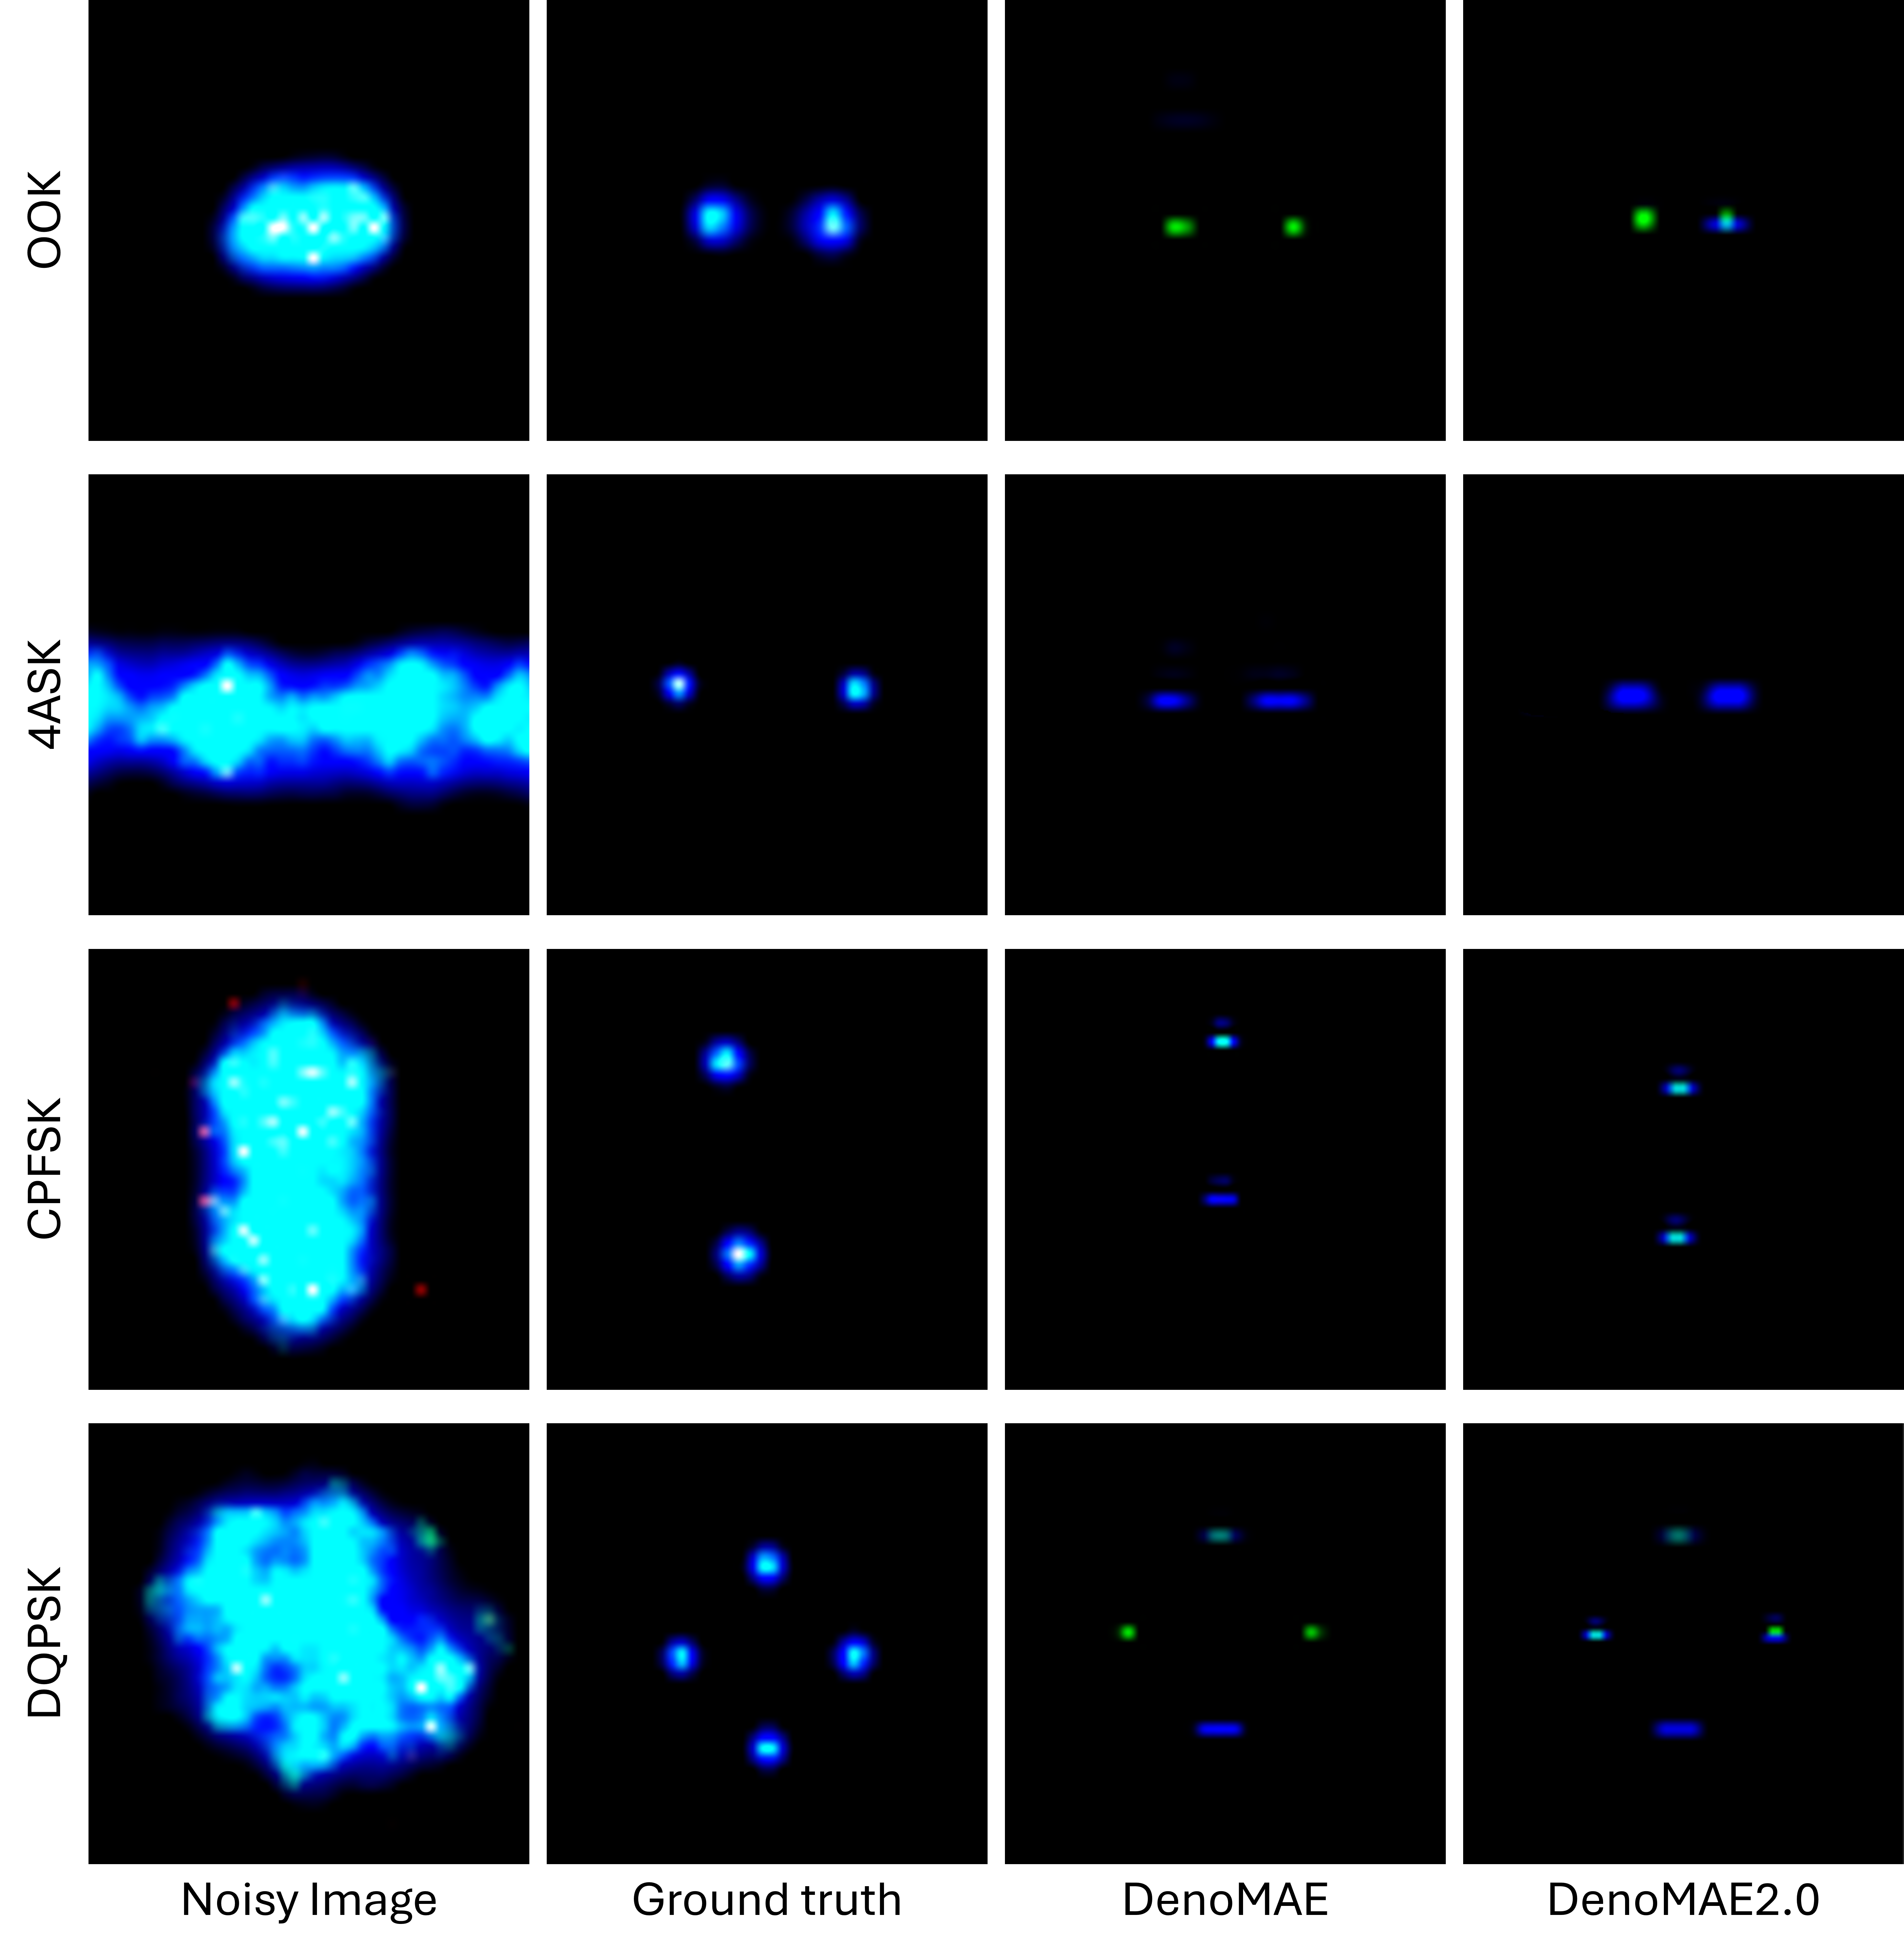
\includegraphics[width=0.7\linewidth]{images/recon.png}
    \caption{Reconstruction}
    \label{fig:recon}
\end{figure*}

The denoising effectiveness of DenoMAE2.0 is evident in the reconstructed constellation diagrams shown in Figure \ref{fig:recon}. Compared to DenoMAE, DenoMAE2.0 achieves superior noise reduction while preserving key signal features crucial for modulation classification. Table \ref{tab:ssim_psnr_comparison} quantifies this improvement using two standard metrics: structural similarity index (SSIM) and peak signal-to-noise ratio (PSNR). Interestingly, for the first image, DenoMAE achieved higher SNR and PSNR despite DenoMAE2.0 producing a visually superior reconstruction. However, for the remaining two samples, DenoMAE2.0 outperformed DenoMAE in both SSIM and PSNR (dB).

\begin{table}[htbp]
    \centering
    \renewcommand{\arraystretch}{1.2}
    \begin{tabular}{|c|c|c|c|}
        \hline
        Method & Image & DenoMAE & DenoMAE2.0 \\ \hline
        \multirow{3}{*}{SSIM} 
        & Image1 & 0.9660 & 0.9634 \\ 
        & Image2 & 0.9407 & 0.9607 \\ 
        & Image3 & 0.9422 & 0.9466 \\ \hline
        \multirow{3}{*}{PSNR (dB)} 
        & Image1 &  42.9054 & 42.3228 \\ 
        & Image2 & 42.0005 & 42.1061 \\ 
        & Image3 & 40.3067 & 40.7508 \\ \hline
    \end{tabular}
    \caption{Comparison of SSIM and PSNR for DenoMAE and DenoMAE2.0}
    \label{tab:ssim_psnr_comparison}
\end{table}

\section{Visualization with TSNE}

\todo[inline]{put tsne here}

\subsection{Finetuning Accuracy}

We compare DenoMAE2.0 with many of the state-of-the-art models to showcase its performance. As shown in Table \ref{tab:example}, DenoMAE2.0 achieves the highest test accuracy of 82.40\% among all compared methods. This represents a significant improvement over the baseline ViT (79.90\%) and other state-of-the-art approaches including DEiT (81.20\%), MoCov3 (81.00\%), BEiT (80.40\%), MAE (80.10\%), and the original DenoMAE (81.30\%). The consistent performance advantage demonstrates the effectiveness of our enhanced denoising strategy for effective representation learning during pretraining.

\begin{table}[htbp]
    \centering
    \resizebox{0.8\linewidth}{!}{%
    \begin{tabular}{|c|c|}
        \hline
        Method & Test accuracy (\%) \\ \hline
        ViT & 79.90 \\ \hline
        DEiT & 81.20 \\ \hline
        MoCov3 & 81.00 \\ \hline
        BEiT & 80.40 \\ \hline
        MAE &  80.10 \\ \hline
        DenoMAE &  81.30 \\ \hline
        DenoMAE2.0 &  \textbf{82.40} \\ \hline
    \end{tabular}%
    }
    \caption{Downstream accuracy.}
    \label{tab:example}
\end{table}

\subsection{Performance on Number of Epochs}

\begin{figure}[htbp]
    \centering
    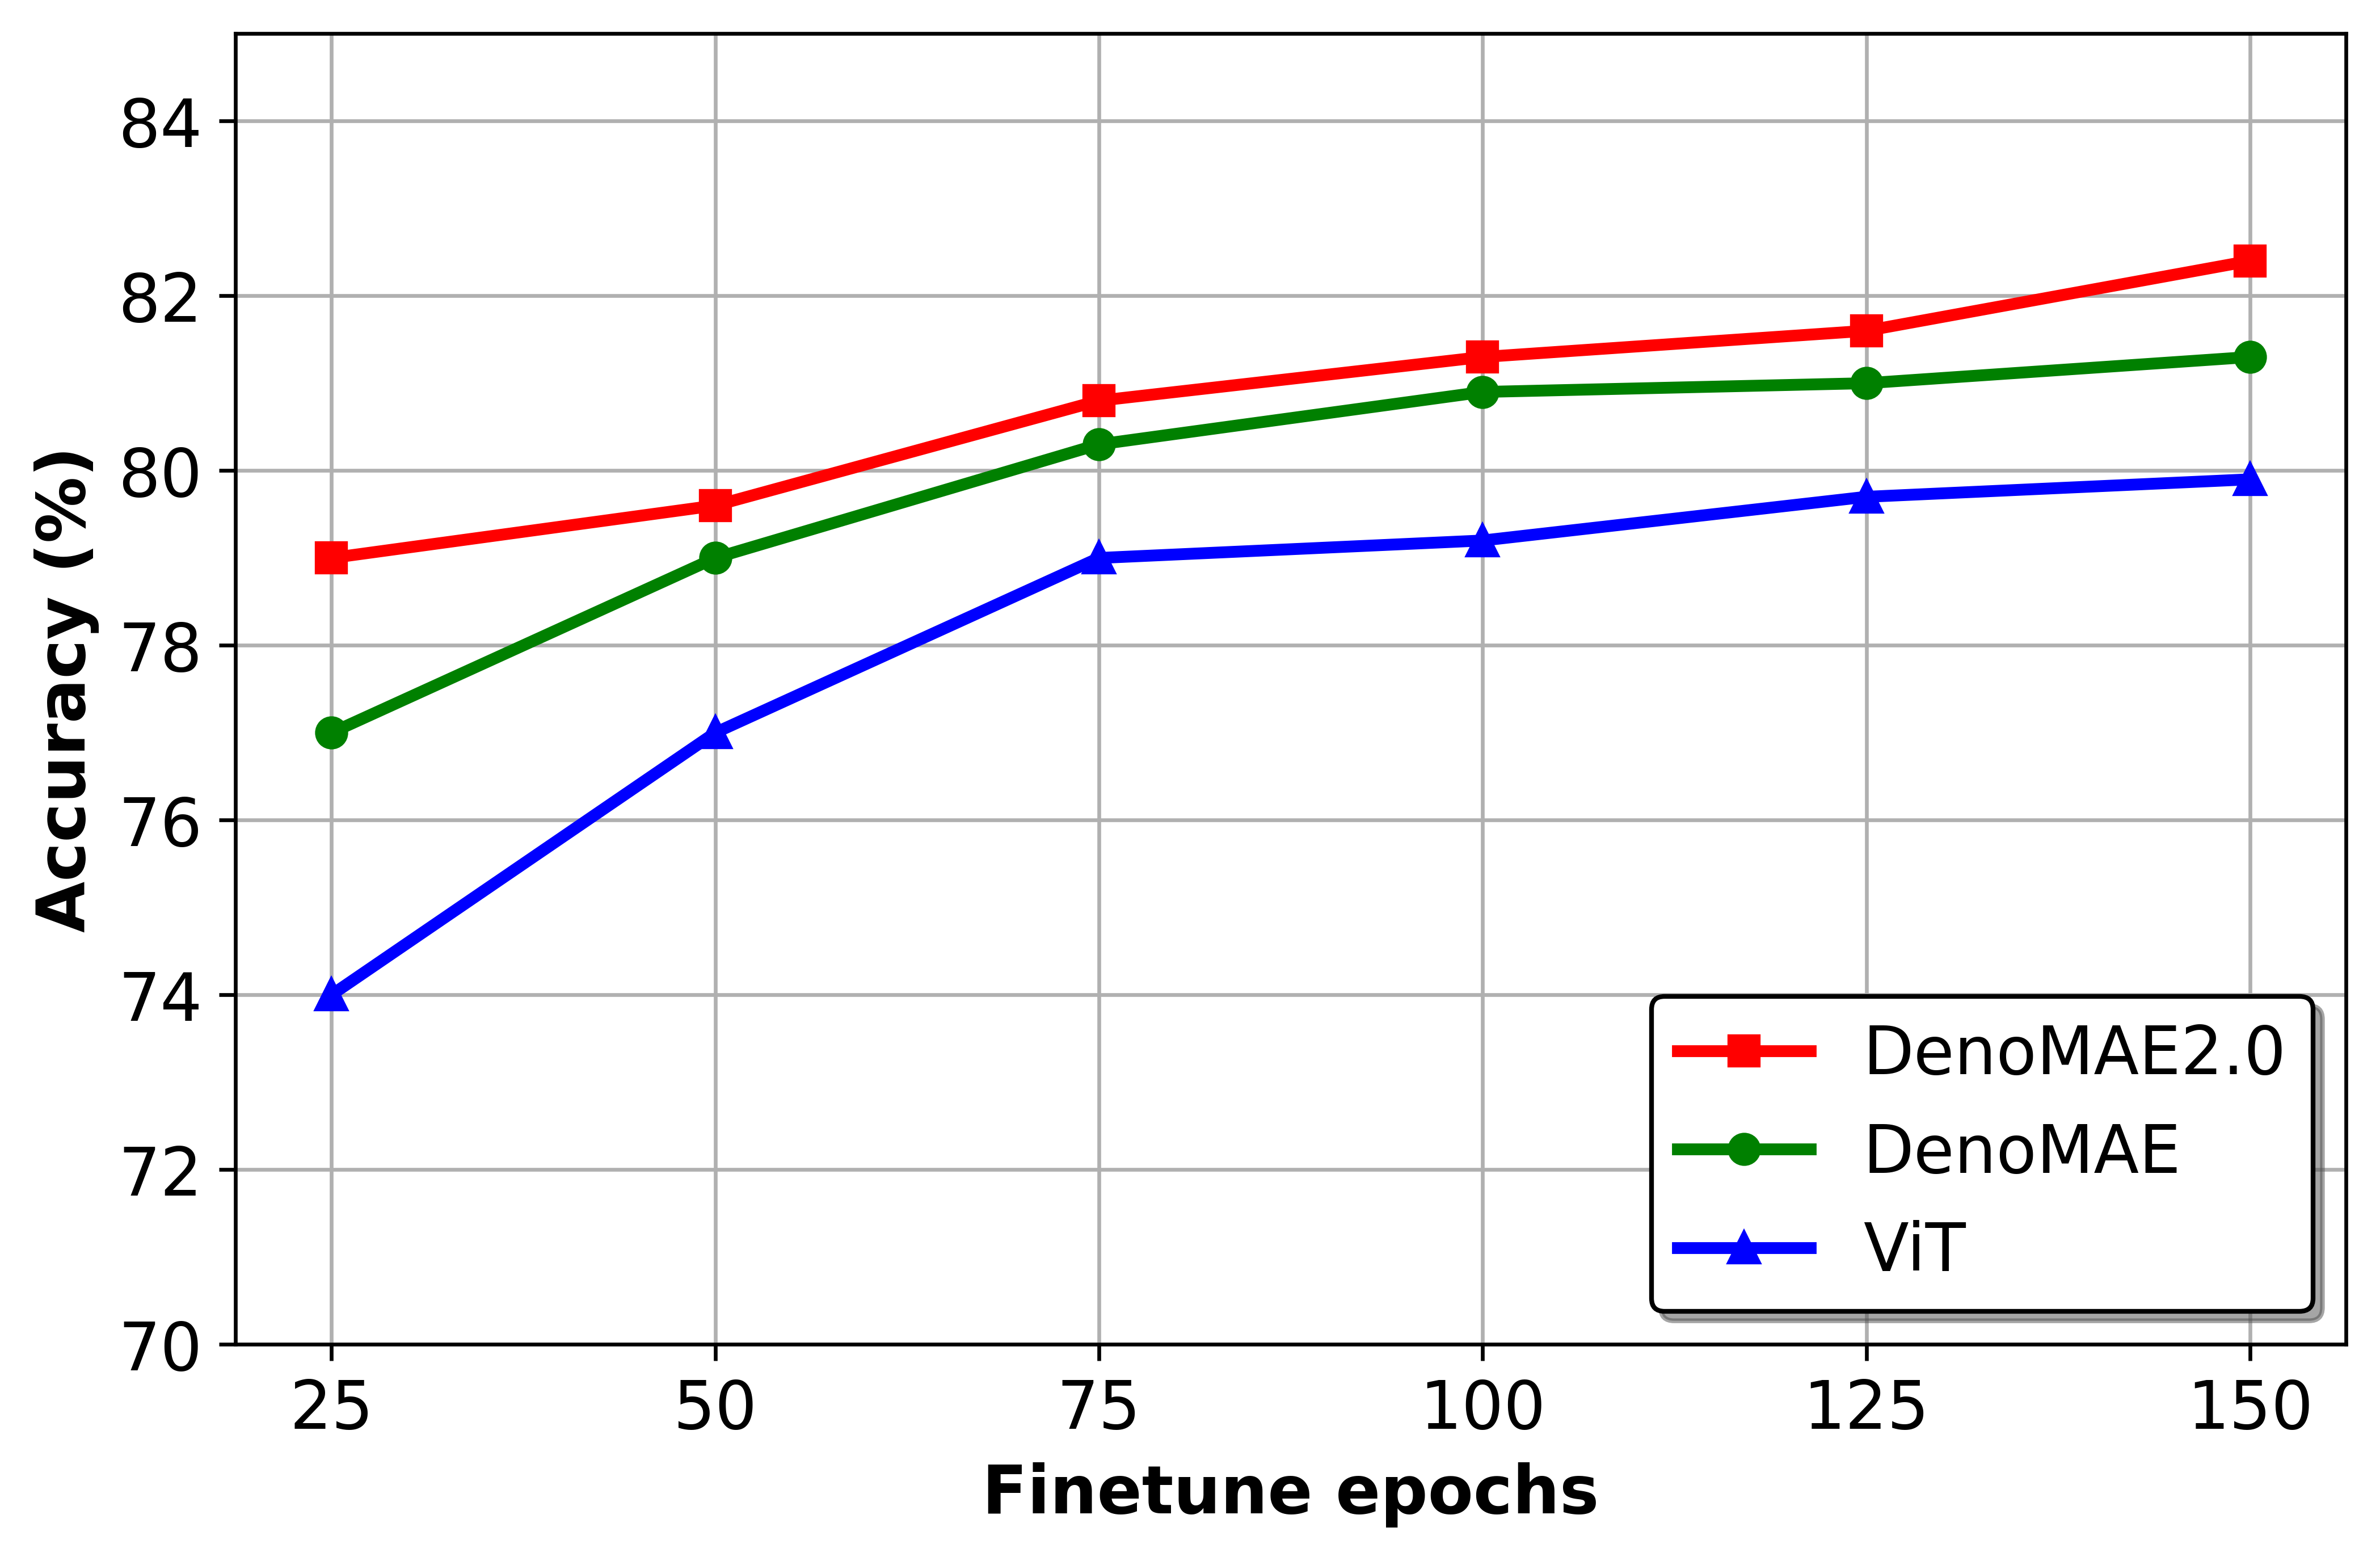
\includegraphics[width=0.9\linewidth]{images/finetune_epoch.png}
    \caption{Epoch finetuning.}
    \label{fig:epoch}
\end{figure}

Figure \ref{fig:epoch} illustrates the finetuning performance across different epochs. The plot shows a steady improvement in model accuracy as the number of epochs increases, with DenoMAE2.0 consistently outperforming baseline methods. DenoMAE achieves higher accuracy than ViT continuously. On the other hand, although the gap between DenoMAE and ViT is larger than DenoMAE and DenoMAE2.0, DenoMAE2.0 always obtains better accuracy than DenoMAE.

\subsection{Performance Across Different SNRs}

The SNR performance plot demonstrates robust classification accuracy across various SNRs ranging from -10 dB to 10 dB. As the SNR values increases all the methods perform better and when the SNR is low the performance degrades. ViT, which has no pertaining phase, presumably obntains the lowest performance in all cases. MAE, which pretrains on modulation signals but has no denoising capability, obtains a slight higher accuracy than ViT. DenoMAE obtains higher accuracy than MAE in most cases however for SNE of 2 and 3 we observe that MAE obtains higher accuracy. On the other hand, DenoMAE2.0 outperforms all the methods for all the SNRs.  Noteably, all the methods lose significant accuracy for snr lower than -2 dB. However, DenoMAE2.0 keeps on a comparatively acceptable accuracy till -7 db. All these outputs indicates DenoMAE2.0's superiority for a more effective representation and ropbustness.



\begin{figure}[htbp]
    \centering
    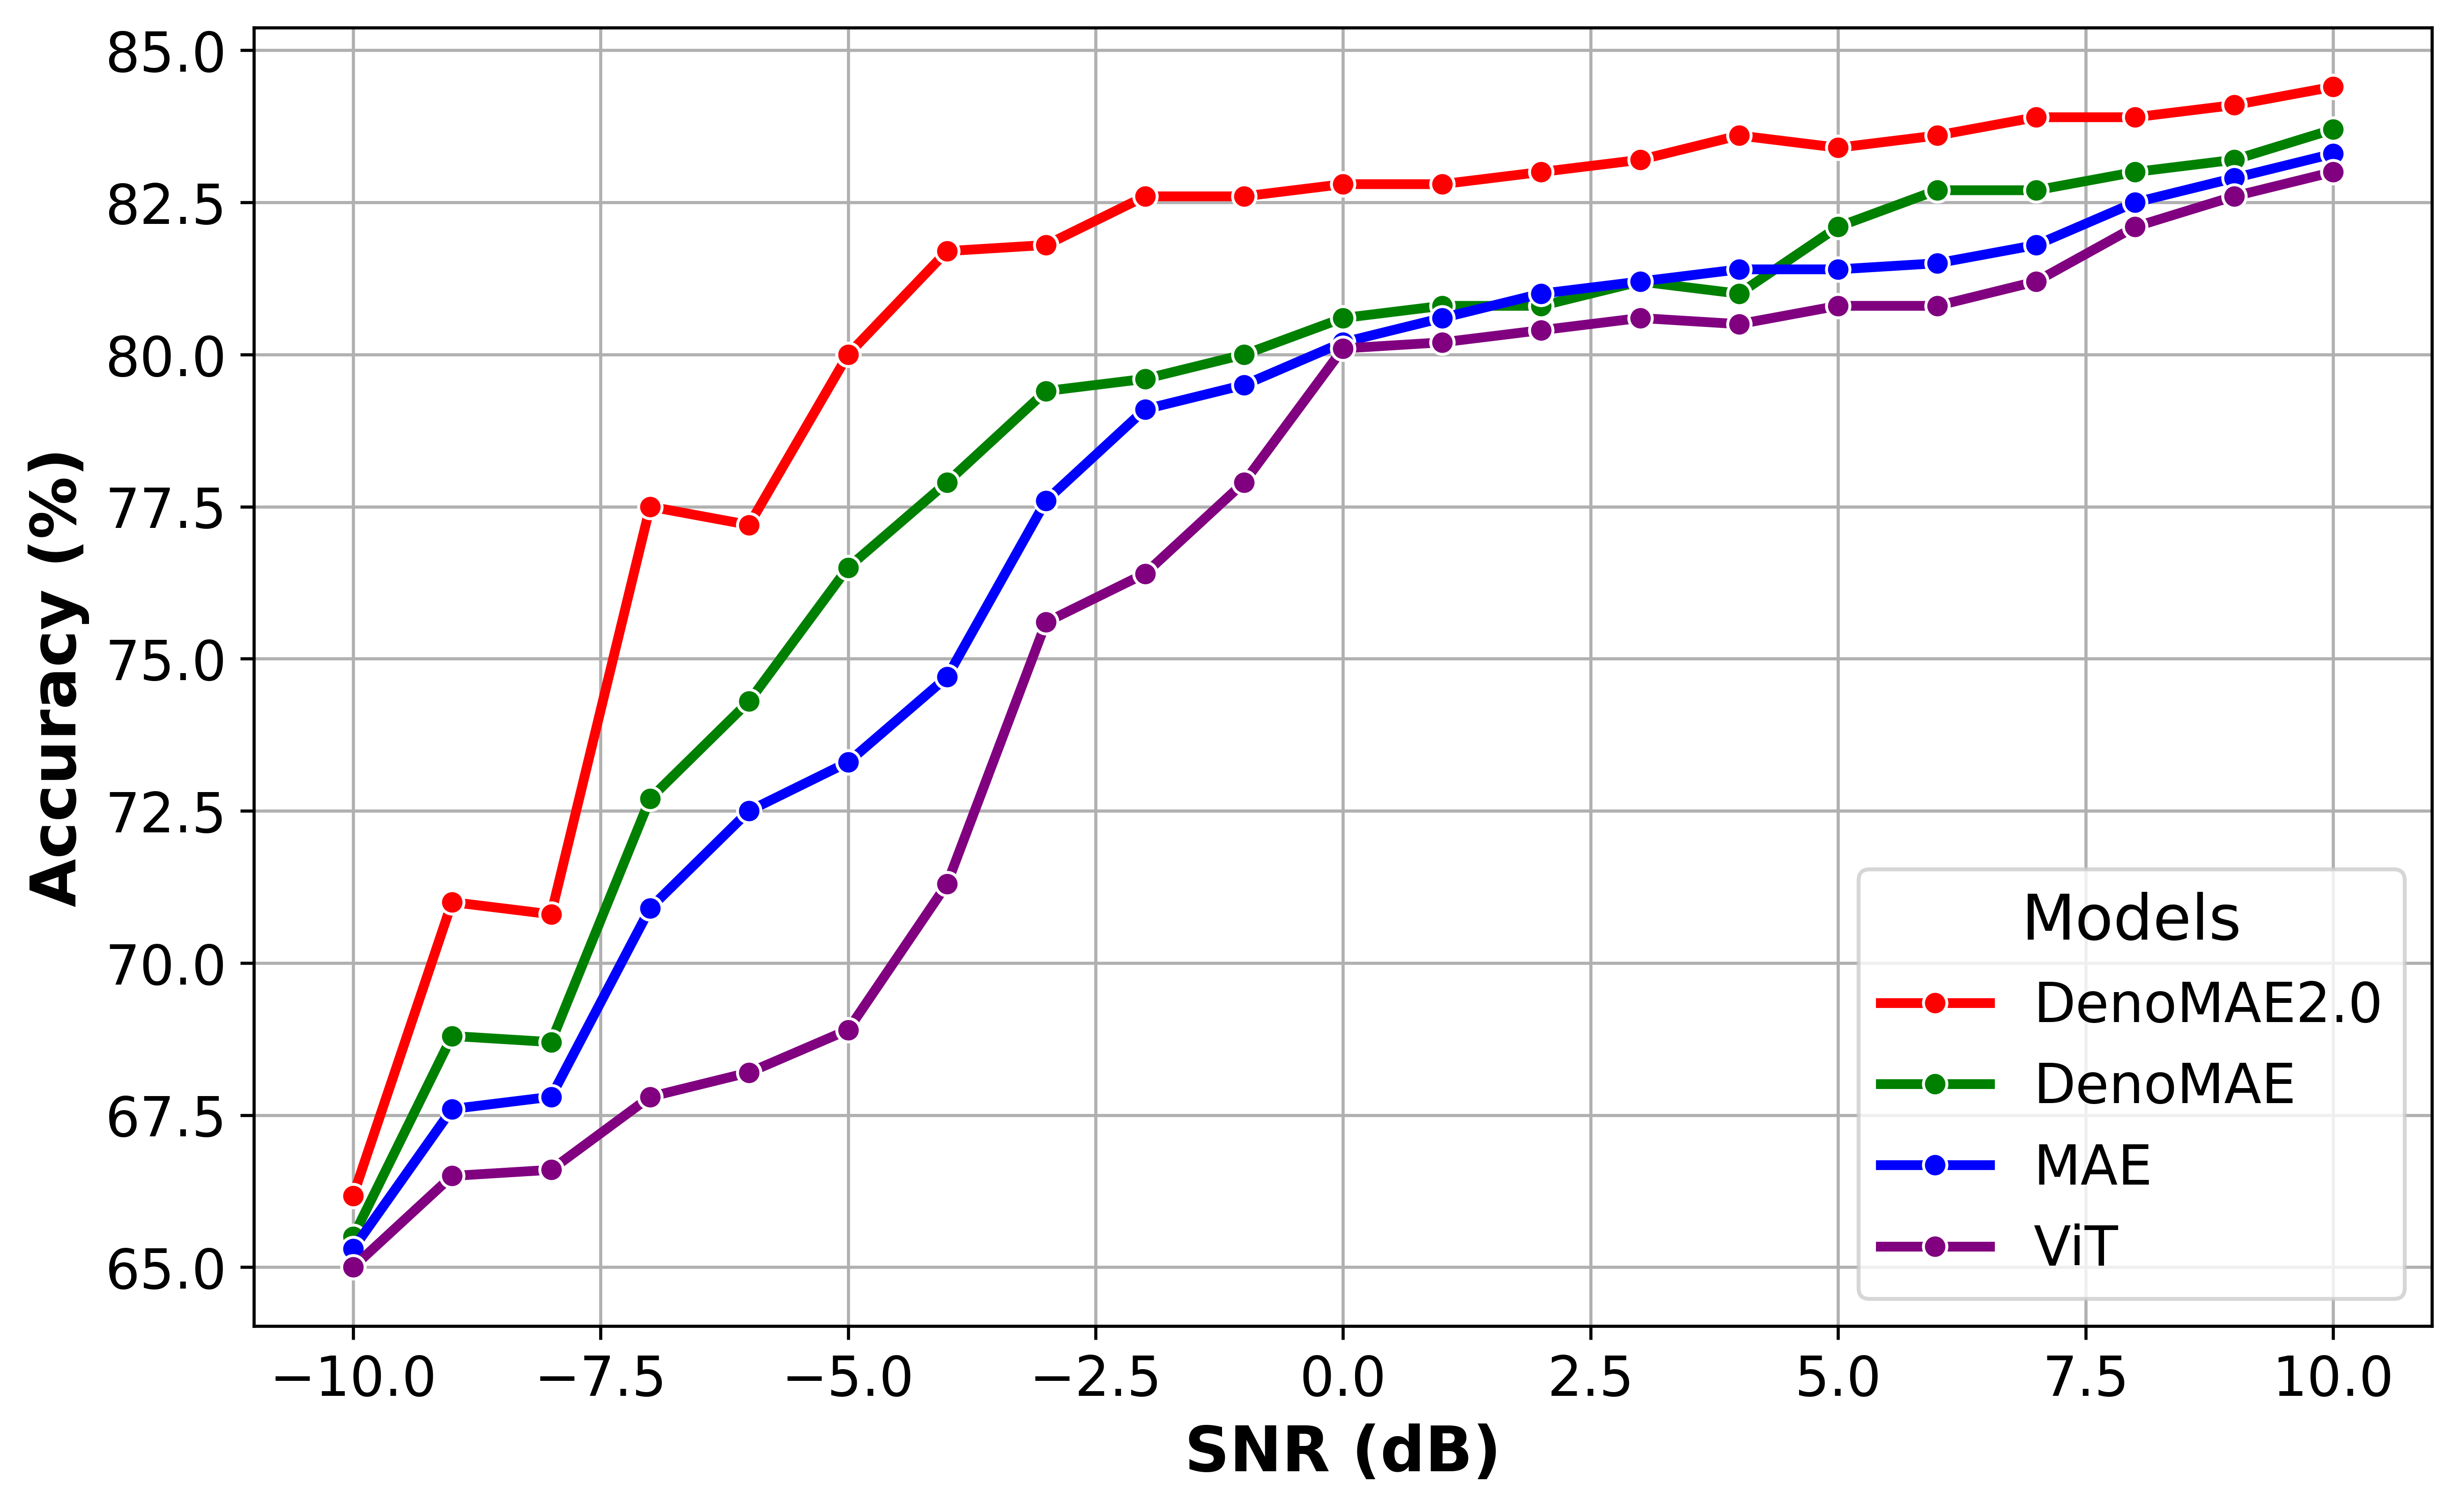
\includegraphics[width=\linewidth]{images/SNR_Accuracy_Plot.png}
    \caption{SNR}
    \label{fig:denomae2}
\end{figure}


\subsection{Transferability}

To show the transferability of DenoMAE2.0 on other similar task, we performed experiments on a similar benchmark dataset named RadioML. A brief description on the RadioML dataset is provided in the following subsection.

\subsubsection{RadioML Dataset}

RadioML 2018.01A \cite{o2018over} is a large-scale dataset designed for automatic modulation classification (AMC) and machine learning-based RF signal processing. It consists of 2,555,904 IQ (in-phase and quadrature) signal samples, where each sample is represented as a 1024×2 array, capturing both in-phase and quadrature components. The dataset spans 24 modulation types, including digital and analog schemes such as BPSK, QPSK, 8-PSK, 16-QAM, AM, and FM, making it a comprehensive resource for signal classification tasks. Signals are generated under 26 distinct signal-to-noise ratio (SNR) levels, ranging from -20 dB to +30 dB in 2 dB increments, simulating real-world conditions affected by fading, interference, and channel noise. Each modulation type and SNR combination contains 4096 samples, ensuring a balanced distribution for model training and evaluation. The dataset, widely used as a benchmark in wireless communication and spectrum sensing research, facilitates advancements in deep learning-based modulation recognition, interference mitigation, and cognitive radio applications.

To keep a consistent same scale implementation, we used 100 samples in each class for the 24 classes in RadioML for training and 10 samples in each class for testing. Therefore, we used only 2400 samples for training and 240 samples for testing. As a result we only used 0.103\% of the total dataset. We only obtain SNRs of -20, -10, 0, 10, 20 dB to show performance across low and high SNRs, as well as interpolaribility. 

\subsubsection{Performance}

The transfer learning capabilities of DenoMAE2.0 are depicted in Figure \ref{fig:trans}. All the methods perform better as the SNR increases and DenoMAE2.0 outperforms all the methods for all the SNRs. DenoMAE2.0 achieves the highest accuracy of 33.75\% for 20 dB SNR where as the closest accuracy obtained by DenoMAE is 21.92\% for 20 dB SNR. This indicates a high accuracy gain of 11.83\% for DenoMAE2.0. Similartly, for SNR of 10 dB, DenoMAE2.0 obtains an accuracy of 29.88\% where as the closest accuracy obtained by DenoMAE is 13.33\%. This indicates a high accuracy gain of 16.55\% more for DenoMAE2.0. As the SNR  decreases and goes out of bound of our pretraining, that is -10 db and -20 db, ViT fails to obtain a meaningful accuracy, achieves only a accuracy of around pure chance (4.27\%) for 24 classes. DenoMAE achieves a slightly improved accuracy than pure chance. However, DenoMAE2.0 achieves a significant accuracy of 7.08\% for -10 db and 6.67\% for -20 db. Therefore, DenoMAE2.0 shows a significant improvement in transferability and robustness for similar tasks.

\begin{figure}[htbp]
    \centering
    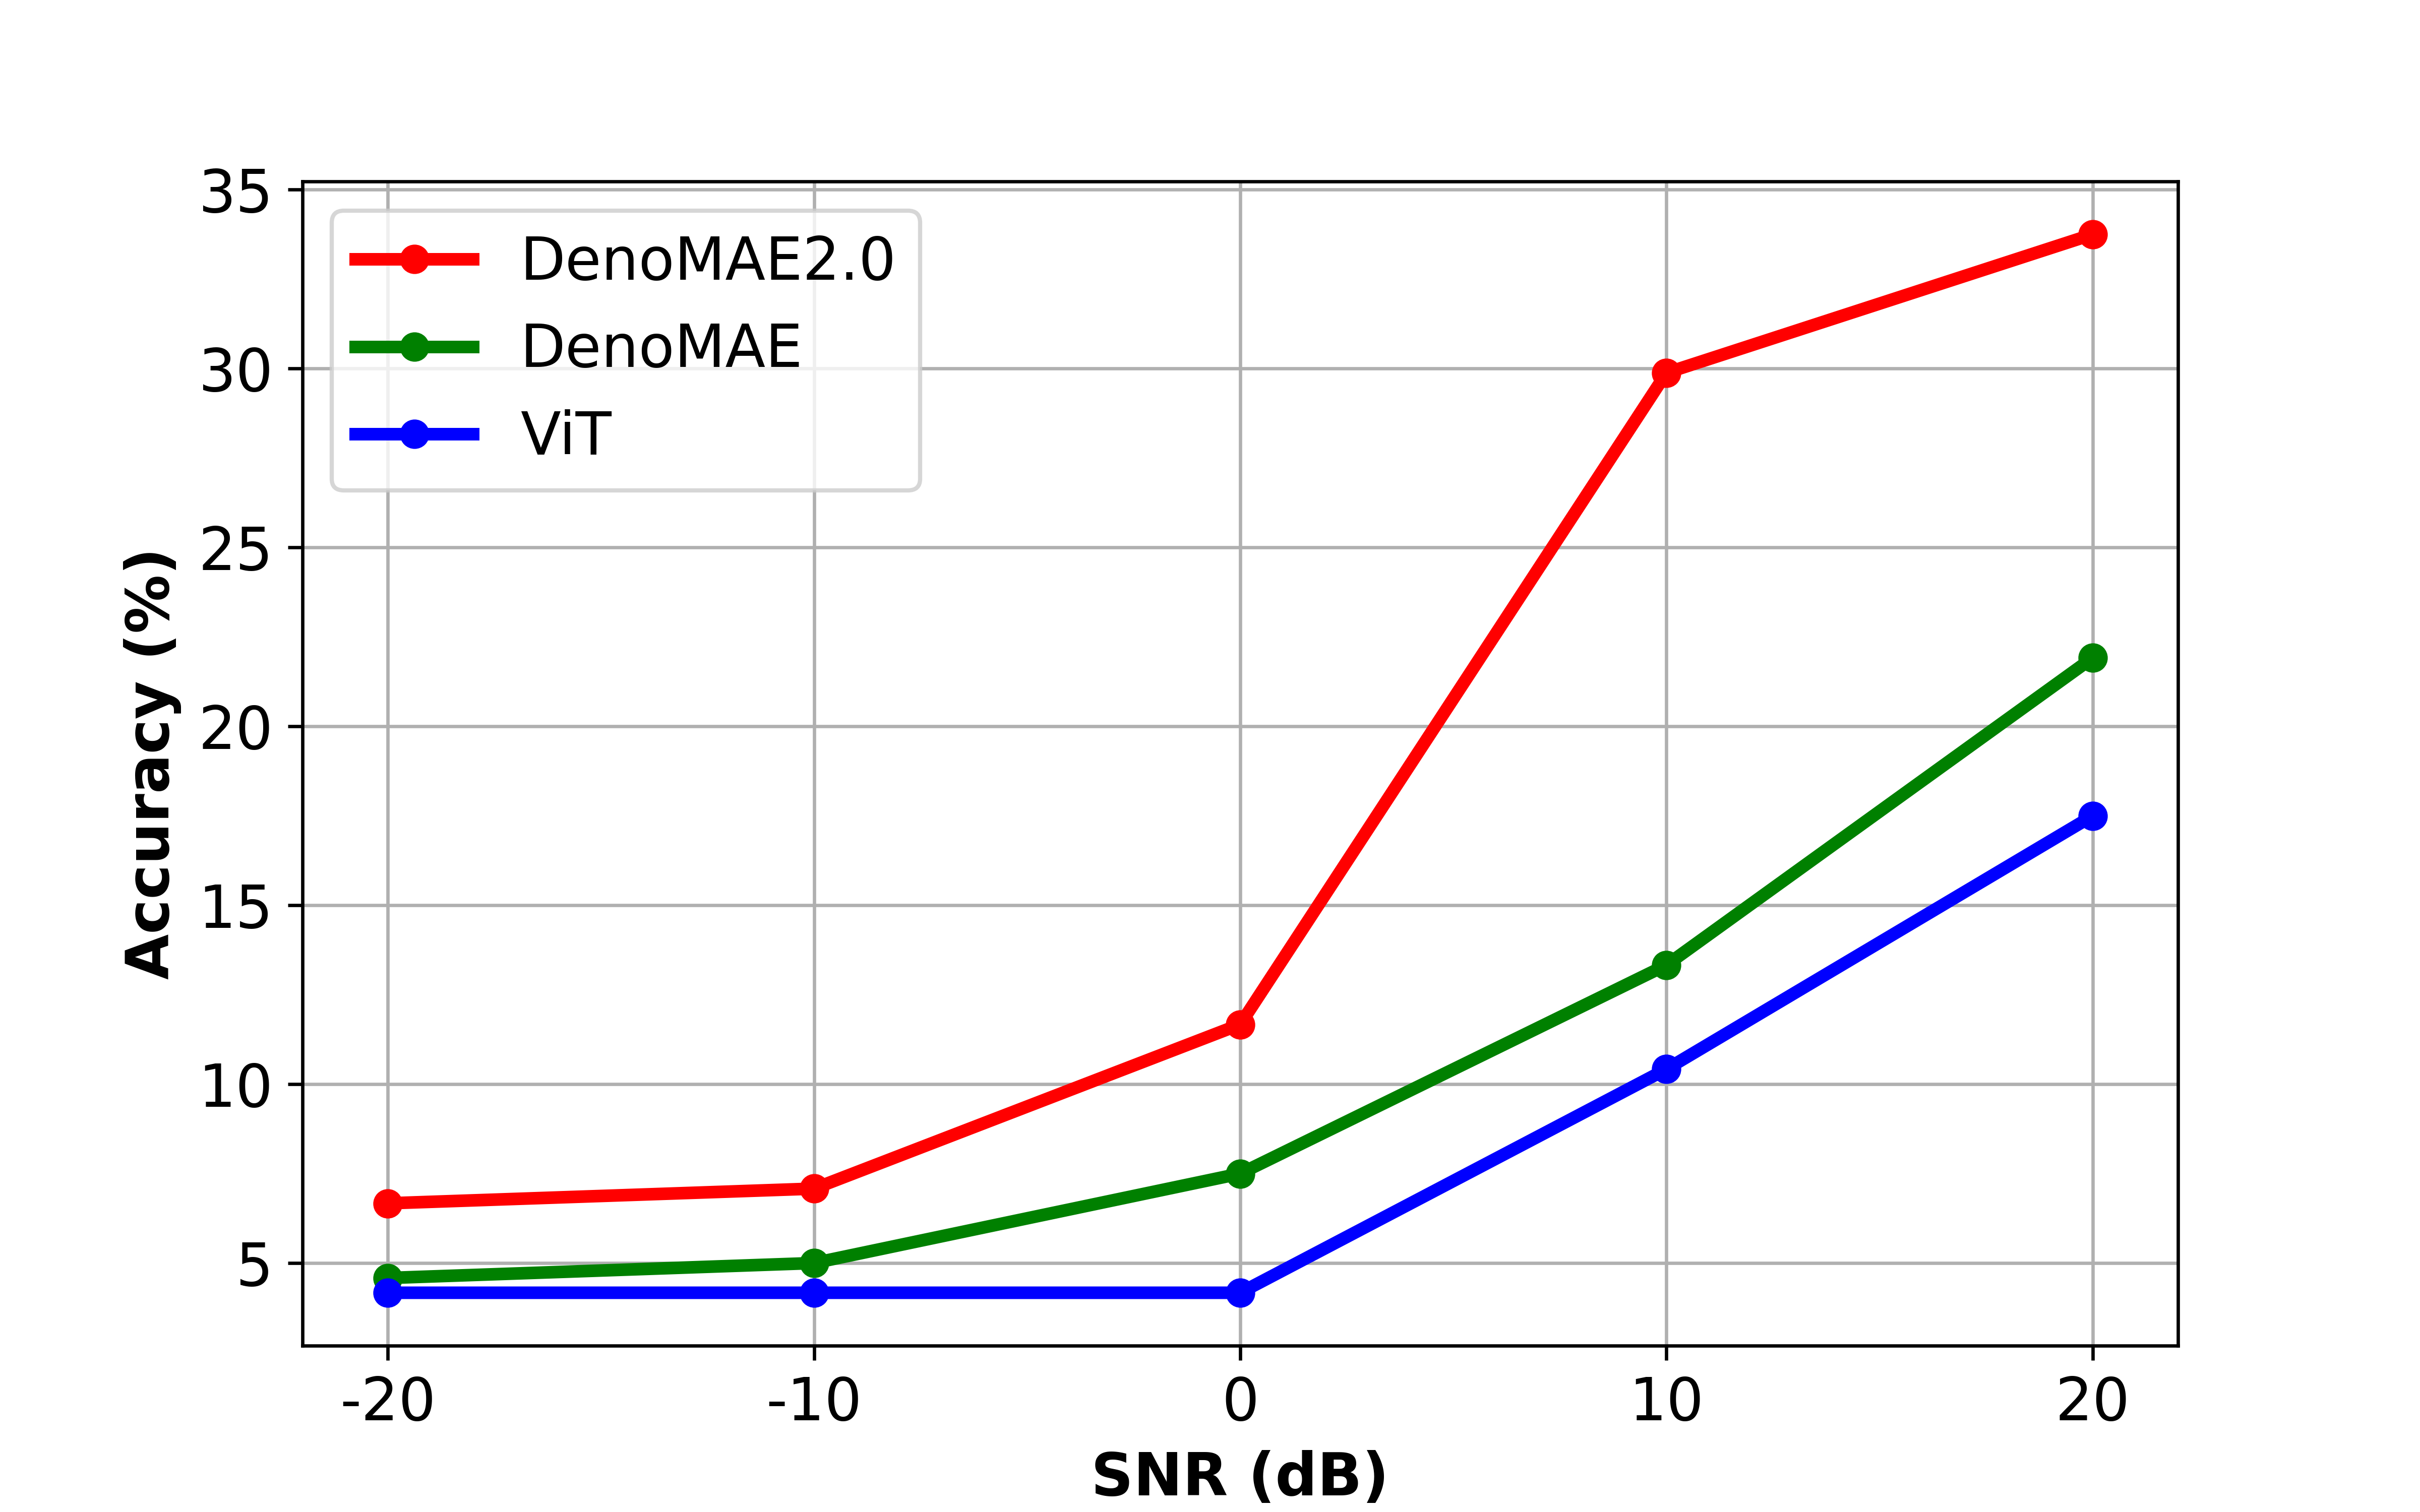
\includegraphics[width=\linewidth]{images/trans.png}
    \caption{Transfer}
    \label{fig:trans}
\end{figure}


\input{chapters/ablation}
\section{Conclusion}

In this work, we presented DenoMAE2.0, an enhanced denoising autoencoder that jointly optimizes reconstruction loss and an unmasked patch classification loss to improve robustness and performance. By incorporating a classification head that refines feature learning on unmasked regions, DenoMAE2.0 surpasses its predecessor, DenoMAE, achieving state-of-the-art results across multiple benchmarks. Extensive experiments demonstrate its superior ability to handle noisy data while preserving high classification accuracy. Additionally, we investigate the influence of auxiliary loss weighting and MLP hidden dimensions on performance, offering key insights into the role of hyperparameter tuning in optimizing denoising autoencoders.  Furthermore, the transfer learning evaluations conducted on the RadioML dataset confirm the superior generalization capabilities of our model across different modulation schemes and varied signal environments. As a result, DenoMAE2.0 presents an efficient and highly effective solution for modulation classification challenges in noisy communication scenarios, showcasing strong potential for real-world wireless communication deployments.




\bibliographystyle{IEEEtran}
\bibliography{references}

\end{document}